\section{Background and Related Works}
\label{sec:background}

\subsection{Software Guard Extension}
\label{sec:background:sgx}

\begin{figure}[t!]
\centering
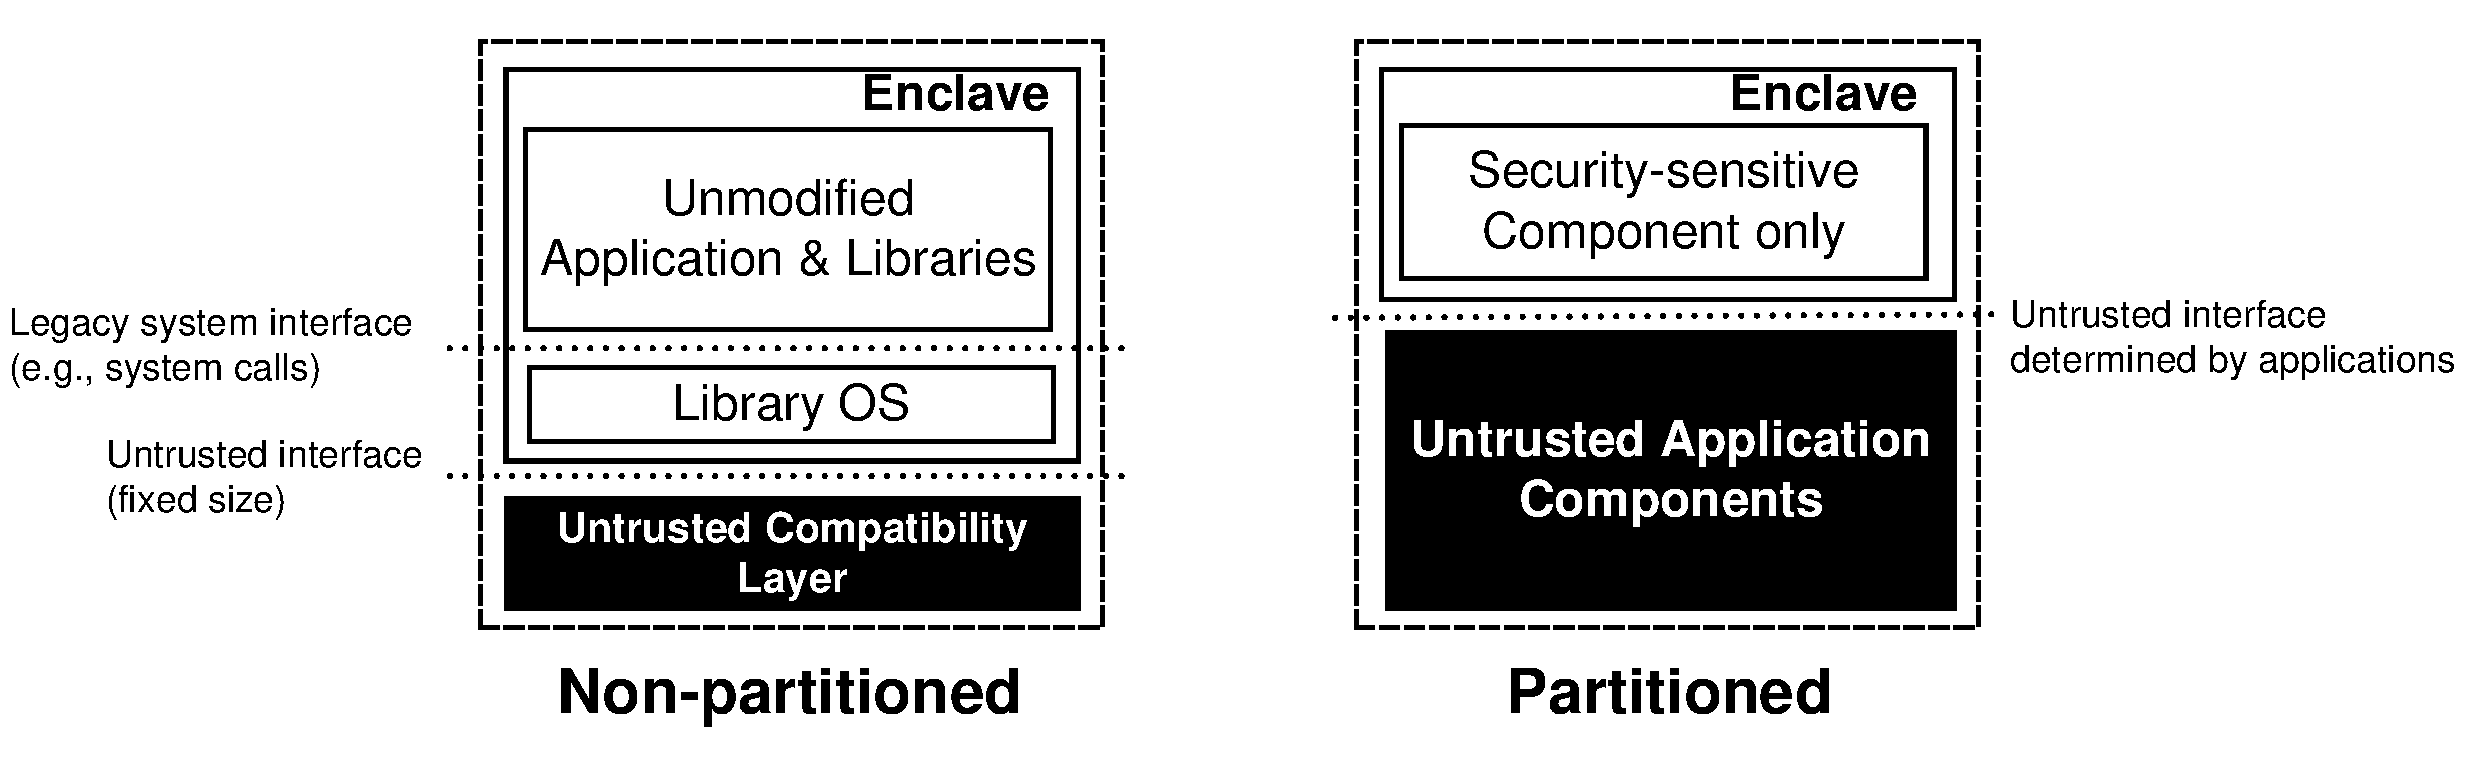
\includegraphics[width=5in]{graphene-sgx/figures/libosvssdk.pdf}
\footnotesize
\vspace{-0.3in}
\caption[Comparison between libOS-based model and partitioned model for Intel SGX]
{Comparison between libOS-based model (e.g., \haven{} and \sysname{})
and SDK-based (SDK for \sgx{}) model for migrating applications in enclaves.
Green (light) boxes are trusted components and red (dark) boxes are untrusted.
The libOS-based model often yields a larger TCB in the enclave,
while the SDK-based model requires developers to be responsible of
securing the enclave on the untrusted interface.}
\label{fig:libosvssdk}
\end{figure}

\sgx{} ({\it Software Guard Extension})
is a set of new x86/x64 instructions
introduced in the latest \intel{} \skylake{} processors,
to create, interface and attest
an isolated memory region (enclave) inside applications' virtual memory.
\sgx{} guarantee any data in an enclave
stay encrypted in the DRAMs, using secret keys derived from
the application's cryptographic measurements.
Security-sensitive information in the enclaves
can only be accessed within the code signed by developers,
who can actively verify that no parts of the code
leak or corrupt the information.

The technology primarily defends applications against two types of attacks:

\begin{compactitem}

\item {\bf From operating system (or hypervisors)}:
Operating systems or hypervisors
that are either compromised by rootkits
or deliberately modified by the host providers.
An attacking host can access the raw data in DRAMs, or remap the
physical pages to other contexts.

\item {\bf Directly on hardware}:
Ones who physically access the hosts can either peep
the DRAM using techniques like cold-boot attacks~\citep{halderman09coldboot},
or intrude the boot process using counterfeit peripheral devices
~\citep{hudson15thunderstrike}.

\end{compactitem}

The use cases of \sgx{} mostly involve the process that an enclave
retrieves a signed attestation from the processor,
to exchange provisioning of critical information from remote servers.
The purpose of such process is equivalent to
expanding the trusted execution
from remote servers
to untrusted hosts,
to harness resources such as CPU cycles and DRAMs.

%One must note that \sgx{} only promises the integrity of application binaries
%initially loaded in enclaves.
%The gap between integrity of binaries and complete security has to be filled
%by ones who develop and approve the applications.
%More specifically, the clients are responsible of
%testing whether the applications contain any vulnerabilities
%that lead to information leak.
%To minimize the risk of leaving any flaws in the applications unintentionally,
%developers often tend to cut down the trusted computing base (TCB)
%of the applications. With smaller TCB, clients who launched the enclaves
%can more easily reason about the thoroughness of securing the execution.

To achieve smaller TCB, the software development kit of \sgx{}
intends to encourage developers to partition the applications and
keep only security sensitive components in the enclaves.
Such an intention is exactly contradicted by the trust model of \haven{},
which must trust the loaded application as a whole.
Except for the cases in which the whole applications must be secured,
\haven{} actually downgrades the trustworthiness of enclaves.
Figure~\ref{fig:libosvssdk} shows the comparison of the two models.

\subsection{Library OSes in \sgx{} Enclaves}
